\chapter{Домашнее задание}

\section{Листинг}

Ниже приведен листинг рассматриваемого в данном случае фрагмента кода.

\begin{code}
\caption{Листинг рассматриваемого кода}
\label{code}
\begin{minted}{C}
for (int y = 0; y < height; y++) {                                  // 1
    for (int x = 0; x < width; x++) {                               // 2
        ray.direction = (QVector3D(x, y, 0) - camera).normalized(); // 3
        colorBuffer[y][x] = traceRay(ray);                          // 4
    }
}
\end{minted}
\end{code}

Внешние данные, такие как \texttt{height}, \texttt{width}, \texttt{camera}, \texttt{colorBuffer} далее будут рассмотрены как константные, так как не изменяются в данном фрагменте кода.

\section{Граф управления}
На рис. \ref{img:1} представлен граф управления для фрагмента кода из листинга~\ref{code}.

\noindent
\begin{figure}[h!]
	\centering
    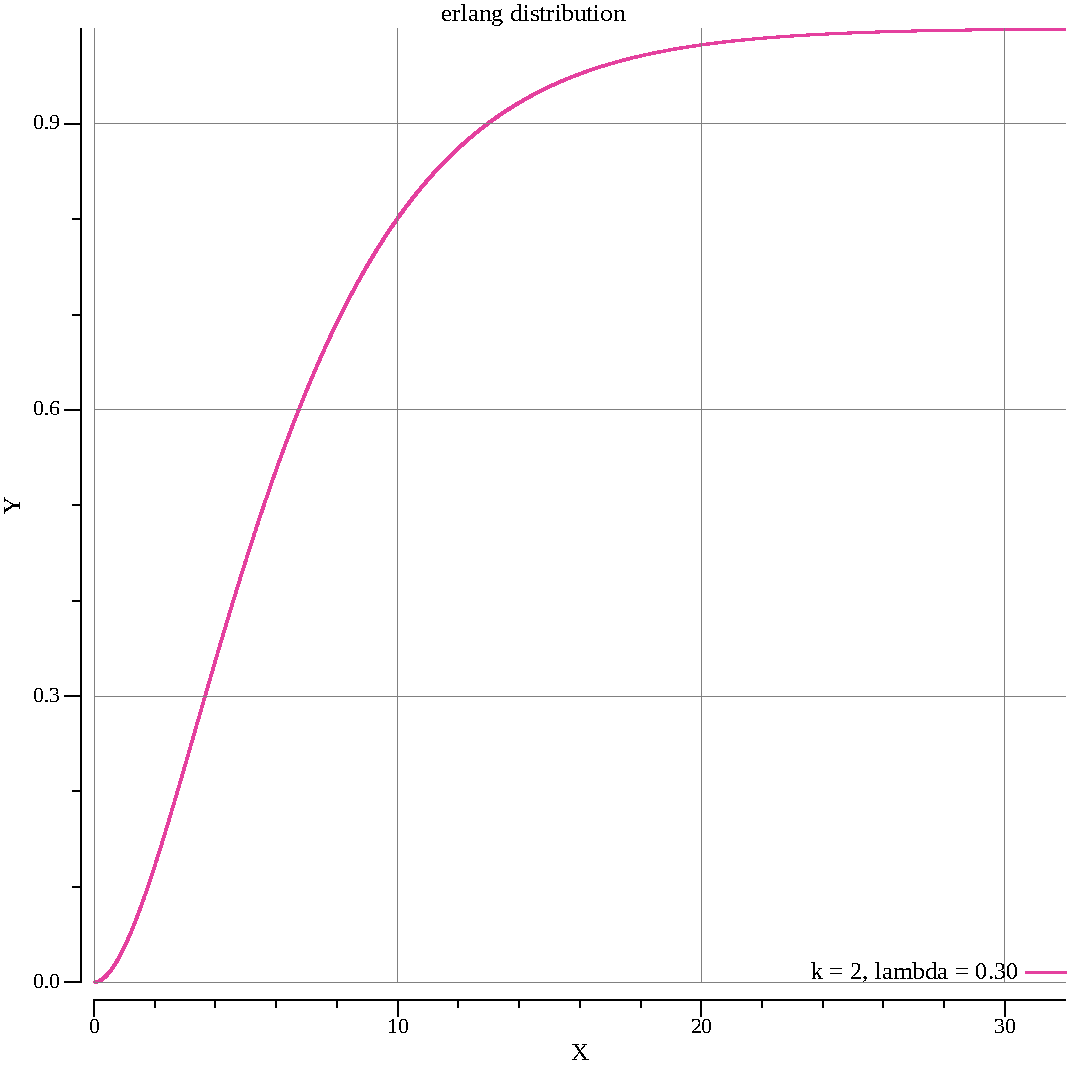
\includegraphics[width=0.12\linewidth]{1}
    \caption{Граф управления}
    \label{img:1}
\end{figure}

\newpage

\section{Информационный граф}
На рис. \ref{img:2} представлен информационный граф для фрагмента кода из листинга~\ref{code}.

\noindent
\begin{figure}[h!]
	\centering
    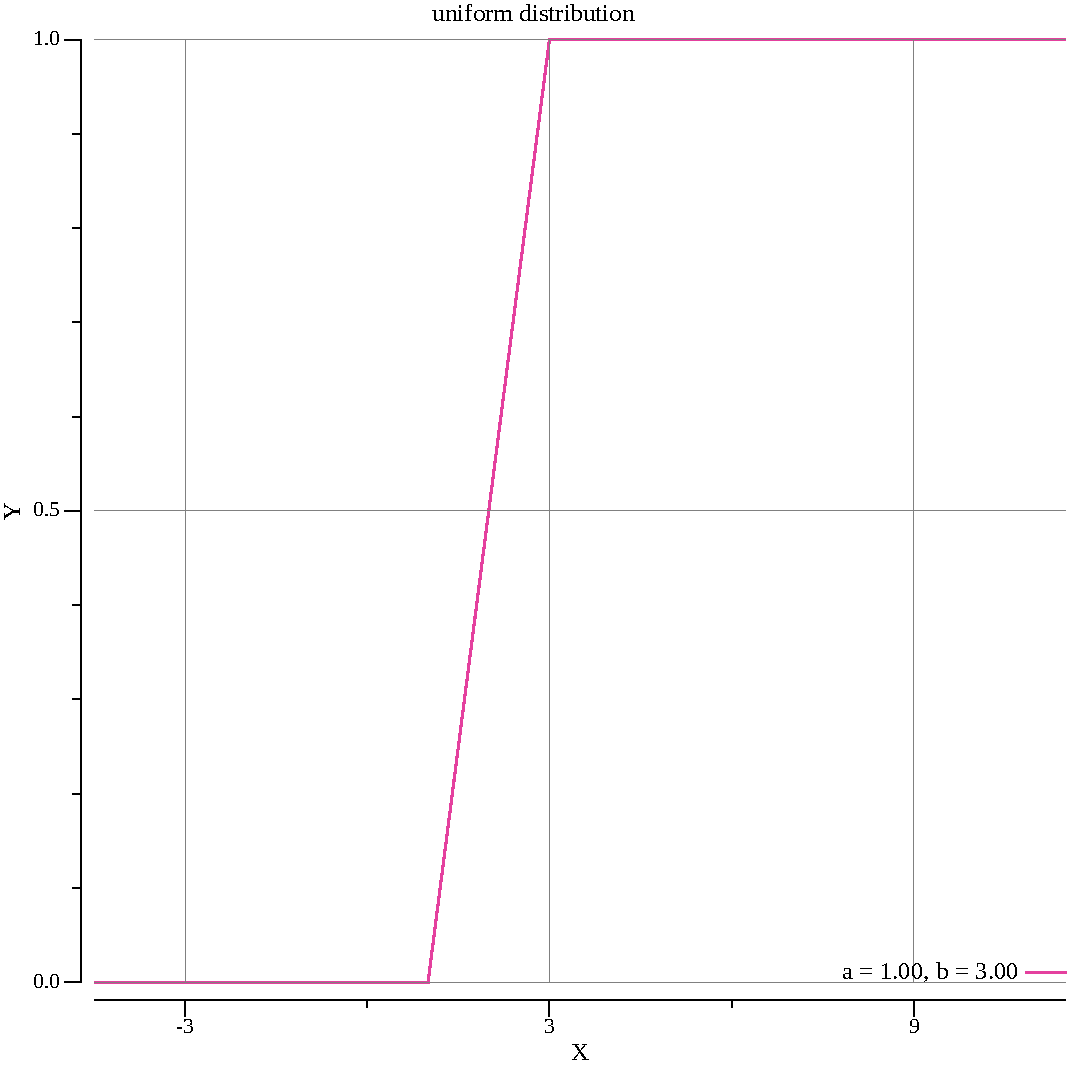
\includegraphics[width=0.1\linewidth]{2}
    \caption{Информационный граф}
    \label{img:2}
\end{figure}

\section{Операционная история}
На рис. \ref{img:3} представлена операционная история для фрагмента кода из листинга~\ref{code}.

\noindent
\begin{figure}[h!]
	\centering
    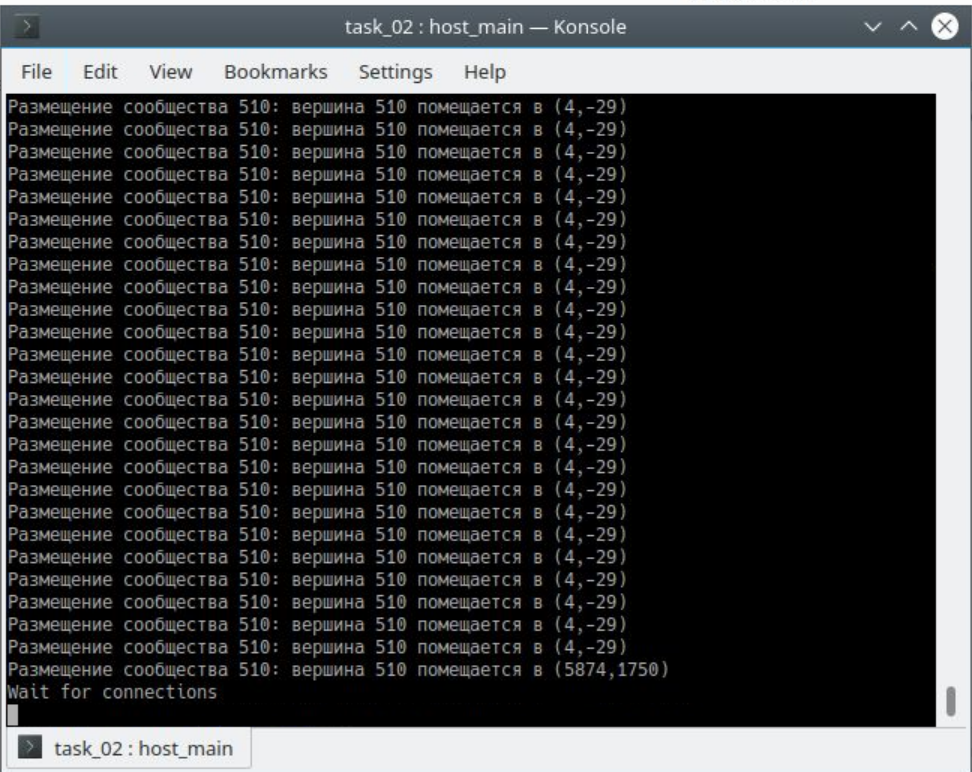
\includegraphics[width=1\linewidth]{3}
    \caption{Операционная история}
    \label{img:3}
\end{figure}

\section{Информационная история}
На рис. \ref{img:4} представлена информационная история для фрагмента кода из листинга~\ref{code}.

\noindent
\begin{figure}[h!]
	\centering
    \includegraphics[width=1\linewidth]{4}
    \caption{Информационная история}
    \label{img:4}
\end{figure}

\newpage